\tikzsetnextfilename{subsequence_posterior}
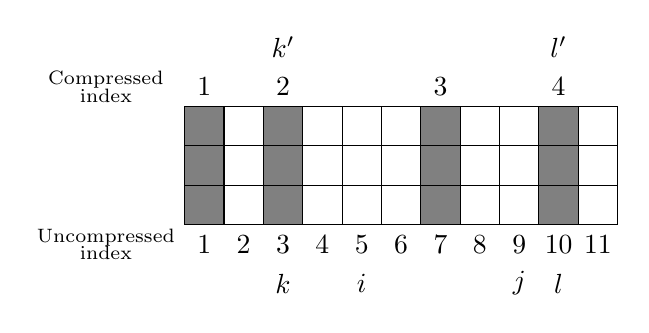
\begin{tikzpicture}
  [scale=0.5]
  \tikzstyle{box} = [draw=black, minimum width=5mm, minimum height=5mm];
  \tikzstyle{gray_box}  = [box, fill=gray];
  \tikzstyle{white_box} = [box];


  \node at (2, 4) {$k'$};
  \node at (9, 4) {$l'$};

  \node[gray_box]  at (0, 0) {};
  \node[gray_box]  at (0, 1) {};
  \node[gray_box]  at (0, 2) {};

  \node[white_box]  at (1, 0) {};
  \node[white_box]  at (1, 1) {};
  \node[white_box]  at (1, 2) {};

  \node[gray_box]  at (2, 0) {};
  \node[gray_box]  at (2, 1) {};
  \node[gray_box]  at (2, 2) {};

  \node[white_box]  at (3, 0) {};
  \node[white_box]  at (3, 1) {};
  \node[white_box]  at (3, 2) {};

  \node[white_box]  at (4, 0) {};
  \node[white_box]  at (4, 1) {};
  \node[white_box]  at (4, 2) {};

  \node[white_box]  at (5, 0) {};
  \node[white_box]  at (5, 1) {};
  \node[white_box]  at (5, 2) {};

  \node[gray_box]  at (6, 0) {};
  \node[gray_box]  at (6, 1) {};
  \node[gray_box]  at (6, 2) {};

  \node[white_box]  at (7, 0) {};
  \node[white_box]  at (7, 1) {};
  \node[white_box]  at (7, 2) {};

  \node[white_box]  at (8, 0) {};
  \node[white_box]  at (8, 1) {};
  \node[white_box]  at (8, 2) {};

  \node[gray_box]  at (9, 0) {};
  \node[gray_box]  at (9, 1) {};
  \node[gray_box]  at (9, 2) {};

  \node[white_box]  at (10, 0) {};
  \node[white_box]  at (10, 1) {};
  \node[white_box]  at (10, 2) {};

  \node[align=center] at (-2.5, 3) {\scriptsize Compressed \\[-2mm] \scriptsize index};

  \node at (0, 3) {1};
  \node at (2, 3) {2};
  \node at (6, 3) {3};
  \node at (9, 3) {4};

  \node[align=center] at (-2.5, -1) {\scriptsize Uncompressed \\[-2mm] \scriptsize index};

  \node at (0, -1) {1};
  \node at (1, -1) {2};
  \node at (2, -1) {3};
  \node at (3, -1) {4};
  \node at (4, -1) {5};
  \node at (5, -1) {6};
  \node at (6, -1) {7};
  \node at (7, -1) {8};
  \node at (8, -1) {9};
  \node at (9, -1) {10};
  \node at (10, -1) {11};

  \node at (4, -2) {$i$};
  \node at (8, -2) {$j$};

  \node at (2, -2) {$k$};
  \node at (9, -2) {$l$};

\end{tikzpicture}
%%% Local Variables:
%%% mode: latex
%%% TeX-master: "../master"
%%% End:
